\section{Supporting multiple languages}
To have a scalable application it is necessary to easily be able to translate the text to different languages.
For this purpose we have used \textit{i18next}, which is an internationalization framework for JavaScript.
Being an internationalization framework means it allows software to be adapted to several languages through localization.
To do this, it makes use of translation files that define the different translations, known as localization files.
I18next is supported for many different frameworks like React, .NET, Angular and many more \cite{i18next}.
\todo{cite er dead}
Instead of hardcoding the text on every page, we wrap the export of the component in the function \texttt{withTranslations} which injects the function \texttt{t} into the props of the component.
The translation file used for translating is the one corresponding to the language chosen by the user in the header of the system.  

\begin{lstlisting}[caption={Translated header when registering as a user.}, captionpos=b, label={withTranslationsUserForm}]
import { withTranslation } from "react-i18next";

function UserForm(props){
    const { t, classes } = props;

    return (
        <Container maxWidth="sm">
            <div className={classes.paper}>
                <Typography align="center" variant="h4">
                    {t('registerasauser')}
                </Typography>
            ...
    );
}

export default withTranslation()(withStyles(styles)(UserForm))
\end{lstlisting}
\noindent
The translation of the the title on the register page can be seen in \autoref{withTranslationsUserForm}.
The \texttt{withTranslation()} function injects the function t into the props of the \texttt{UserForm} component.
When called, the function t will look up the passed key in the translation files to find the correct translation for \texttt{registerasauser}. 
A screenshot of a snippet of the files can be seen on \autoref{fig:translationfiles}.
\begin{figure}
    \centering
    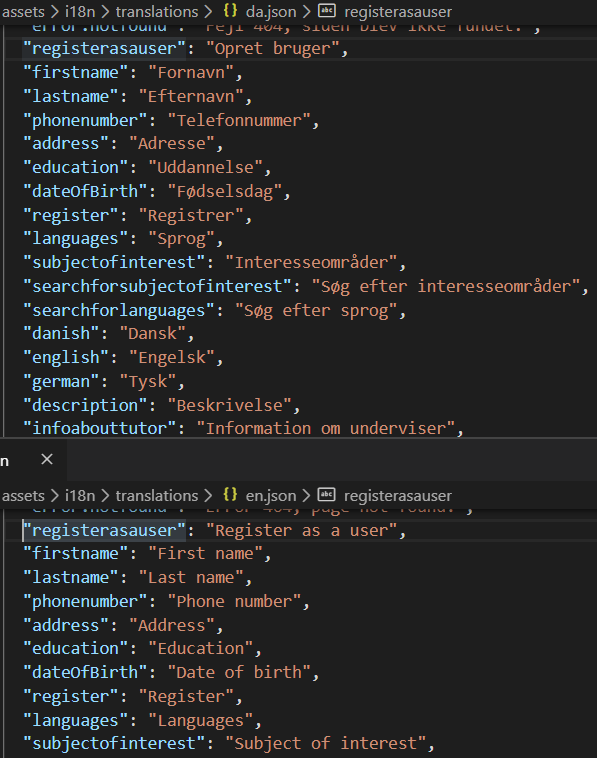
\includegraphics[scale=0.5]{figures/translationexample.PNG}
    \caption{The Danish and English translation files}
    \label{fig:translationfiles}
\end{figure}
\noindent
To add an additional language a new translation file needs to be created.
All the lines that are present in the other files then need to be translated to the desired language. 
It is not necessary to refactor any code to add additional languages.
